\section{Problem Setup}
\label{sec:problemSetup}
In this work, we focus on the particular case of autonomous corridor navigation. For this purpose we use the vanishing point algorithm \cite{VP1}, \cite{VP2} and feedback control to maintain heading parallel to the corridor and stay in the middle of it. We implement the algorithm on a $1/10^{th}$ scale car we developed. The robot is equipped with a front facing camera which feeds image frames to the vanishing point algorithm for processing.The computation platform on board the car is a Nvidia Jetson, which has a quad-core ARM CPU and a 192 core Nvidia Tegra GPU.


\subsection{Vanishing point-based corridor navigation}

The Vanishing point algorithm \cite{VP1} has been used extensively in indoor settings for navigating corridors autonomously \cite{VP2, VP3} and for outdoor lane detection \cite{gallagher2002ground}.
For each image frame processed, the algorithm outputs the horizontal distance of the vanishing point and middle point (for details, refer to \cite{VP1}) from the center of the frame. These two measurement signals are used as feedback by the controller to center and align the robot along the corridor. For more details see Sec. \ref{}[experimental]. Figure \ref{fig:vp_viz} shows a visualization of Vanishing point operating on a frame collected from our robot navigating in a corridor.

\begin{figure}[hbtp]
\centering
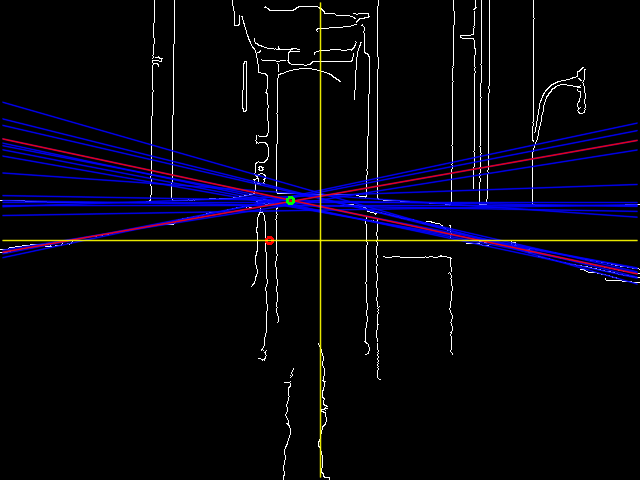
\includegraphics[width=0.46\textwidth]{Figs/vpmpimages/image_23_-30_-51.png}
\caption{Visualization of the Vanishing point algorithm. The green dot shows the vanishing point while the red dot shows the middle point.}
\label{fig:vp_viz} %diff freq same assignment}
\end{figure}

 We define \textit{throughput} of the algorithm as the update rate of the vanishing point algorithm, which is the inverse of its execution time. The faster the vanishing point algorithm executes, the better the control performance of the closed loop system can be since the controller sees a small delay. Hence, throughput acts as a proxy for control performance. In most implementations, the perception algorithm is implemented to run at its maximum possible throughput at all times in order to subject the controller to small delays while the power consumed by the computation platform in doing so is neglected during the design and implementation process. With the computation platform in our setup, we can run the vanishing point algorithm on the CPU or the GPU, and also change the clock frequencies of both the CPU and the GPU. In our implementation, we found that running the vanishing point algorithm on the CPU alone resulted in a low throughput (~8Hz) and low power consumption (~5.2W). On the other hand running it on the GPU allowed us to get a throughput in excess of 20Hz, but resulted in a power consumption of over 7W. In many autonomous systems, power draw from the computation platform is a significant concern, e.g. in our robot the Jetson is powered by an energy source that is separate from the energy source for the drive motors. So while we would want to subject the controller to a small delay (operate the perception algorithm at a high throughput), we would also like to minimize the power draw from the computation platform in order to maximize the operating time of the system. 


\subsection{Exploiting hardware knobs to trade-off computation power and throughput}

In order to trade-off computation power and throughput of the perception algorithm, we rely on the insight that scheduling some tasks on the GPU can in general result in a speed up over executing them on the CPU while consuming more power (see Sec. \ref{}[profiling]. Also, we can also get a speed up by increasing CPU and GPU frequencies, but at the cost of increased power draw by the computation platform. In order to achieve a wide range of trade-offs we focus on the major computational tasks that comprise the vanishing point algorithm, which are briefly explained below:

\begin{itemize}
\item Blur: A Gaussian blur is applied on the image for de-noising.
\item Edge detection: We use the Canny Edge detector to find edges in the image.
\item Hough Transform: used to detect straight lines in the image.
\item RANSAC: used to select the parallel straight lines that best describe the sides of the corridor. These lines intersect in the image plane at the Vanishing Point.
\end{itemize}

Note, on the Jetson, we can schedule any of these tasks to be run on either the CPU or the GPU as shown in Fig. \ref{fig:vanishing} In addition, we can also change the CPU and GPU frequencies during run-time, resulting in different execution times for the vanishing point algorithm and different power consumption for the Jetson. Let the schedules for the tasks on the CPU or the GPU be denoted by 

\begin{subequations}
\begin{align}
\sigma&\in\Sigma\text{ where,} \nonumber \\
\Sigma&=\{\text{CCC, CCG, CGC, CGG, GCC, GCG, GGC, GGG}\} \nonumber
\end{align}
\end{subequations}

Here, schedule $\sigma=\text{CCC}$ implies that the Blur tasks is done on the CPU, the Edge detection is done on the CPU and the Hough Transform is done the CPU, $\sigma=\text{CCG}$ implies that the Blur tasks is on the CPU, Edge detection is on the CPU and the Hough Transform is done on the GPU, and so on. Note, since RANSAC took a negligible amount of time compared to the other tasks, we always execute it on the CPU.
Also, denote $F_c$ and $F_g$ to be the frequency of the CPU and the GPU respectively. The hardware level knobs to trade-off throughput and computation power for an execution of the vanishing point algorithm are now $\sigma$, $F_c$ and $F_g$. The throughput and computation power, functions  of all three knobs are denoted by $T(\sigma,F_c,F_g)$ and $P(\sigma,F_c,F_g)$ respectively.

\begin{figure}
	\centering
	\includegraphics[scale=0.3]{Figs/vanishing}
	\caption{The vanishing point algorithm with components running on either CPU or GPU at various frequencies, resulting in different power consumptions and execution times.}
	\label{fig:vanishing}		
\end{figure}

\subsection{Problem statement}
With the hardware level knobs explained and keeping in mind that more throughput means better control performance for the closed loop system, the problem we want to solve is that of picking the best operating mode ($\sigma$, $F_c$ and $F_g$) for the perception algorithm in order to minimize computation power $P(\sigma,F_c,F_g)$ without overly affecting the closed loop control performance of the system, which is related to $T(\sigma,F_c,F_g)$. For this, we propose a two step solution and evaluate it for out problem setup. This is explained in more detail in the following sections.


